\addcontentsline{toc}{chapter}{Занятие 10. Интервальное оценивание параметров.
                              Доверительные интервалы}
\chapter*{Занятие 10. Интервальное оценивание параметров. Доверительные интервалы}

\addcontentsline{toc}{section}{Контрольные вопросы и задания}
\section*{Контрольные вопросы и задания}

\subsubsection*{Приведите определение доверительного интервала с уровнем значимости $ \alpha $,
                ассимпточисеского деверительного интервала с уровени значимости $ \alpha $.}

Имеем семейство распределений $F_{ \theta }$,
зависящее от параметра $ \theta \in \Theta \subset \mathbb{R}$.
Имеем выборку $X_1, \dotsc, X_n$ из распределения $F_{ \theta }$.

Есть две статистики: $T_1$ и $T_2$ такие, что $T_1 \leq T_2$ почти наверное,
то есть это некоторый случайный интервал $ \left[ T_1, T_2 \right] $.
Задаём число $ \alpha \in \left( 0, 1 \right) $, как правило $ \alpha \ll 1$.

Промежуток $ \left[ T_1, T_2 \right] $ ---
это доверительный интервал для $ \theta $ с уровнем доверия $ \alpha $,
если
$ \forall \theta \in \Theta: \,
  P_{ \theta } \left( T_1 \leq \theta \leq T_2 \right) \geq 1 - \alpha $.

Интервал $ \left[ T_1, T_2 \right] $
называется асимптотическим доверительным интервалом для параметра $ \theta $ уровня доверия
$ \alpha $,
если для любого
$$ \theta \in \Theta: \,
  \lim \limits_{n \to \infty } inf \, P_{ \theta } \left( T_1 \leq \theta \leq T_2 \right) \geq
  1 - \alpha.$$

\subsubsection*{Какая статистика называется центральной?}

Функция $G \left( \vec{X}, \theta \right) $ называется центральной статистикой,
если выполняется ряд требований:
\begin{enumerate}
  \item $G \left( \vec{X}, \cdot \right) $ --- функция второго аргумента ---
  строго монотонна и непрерывна (либо строго возрастает, либо строго убывает);
  \item $G \left( \vec{X}, \theta \right) $ имеет известное распределение,
  не зависящее от $ \theta $.
\end{enumerate}

\subsubsection*{Как с помощью центральной статистики построить доверительный интервал с заданным
                уровнем доверия?}

Пусть $G$ --- центральная статистика.
Распределение $G$ --- известно.

Следовательно, по $ \alpha $ можно указать такие числа $a_1 < a_2$, что имеет место следующее:
$P \left\{ a_1 \leq G \left( \vec{X}, \theta \right) \leq a_2 \right\} \geq
  1 - \alpha $.

Считаем, что $G \left( \vec{X}, \cdot \right) $ возрастает.
Тогда это равносильно тому,
что
$$P_{ \theta } \left\{
    G^{-1} \left( \vec{X}, a_1 \right) \leq \theta \leq G^{-1} \left( \vec{X}, a_2 \right)
  \right\}
  \geq 1 - \alpha.$$
Эти границы $G^{-1} \left( \vec{X}, a_1 \right), \, G_2^{-1} \left( \vec{X}, a_2 \right) $ ---
доверительный интервал.

\addcontentsline{toc}{section}{Аудиторные задачи}
\section*{Аудиторные задачи}

\subsubsection*{10.3}

\textit{Задание.}
По выборке $X_1, \dotsc, X_n$ из нормального распределения $N \left( a, \sigma^2 \right) $
постройте доверительные интревалы для параметров распределения, если:
\begin{enumerate}[label=\alph*)]
  \item $a$ неизвестный параметр, $ \sigma^2$ --- известный;
  \item $ \sigma^2$ неизвестный параметр, $a$ --- известный.
\end{enumerate}

\textit{Решение.} С помощью этих распределений можно строить доверительный интервал:
$$ \begin{cases}
    \frac{ \sqrt{n} \left( \overline{X} - a \right) }{ \sigma } \sim N \left( 0, 1 \right), \\
    \frac{ \left( n - 1 \right) \hat{ \sigma^2}}{ \sigma^2} \sim \chi_{n - 1}^2, \\
    \frac{ \sqrt{n} \left( \overline{X} - a \right) }{ \hat{ \sigma }} \sim t_{n - 1}.
  \end{cases}$$

\begin{enumerate}[label=\alph*)]
  \item Используем первое
  $$ \xi =
    \frac{ \sqrt{n} \left( \overline{X} - a \right) }{ \sigma } \sim
    N \left( 0, 1 \right).$$

  Если задан уровень доверия $ \alpha $, по таблице можем найти
  $$P \left( \xi \geq u_{ \frac{ \alpha }{2}} \right) =
    \frac{ \alpha }{2} =
    \Phi \left( u_{ \frac{ \alpha }{2}} \right).$$

  Плотность имеет вид колокольчика,
  поэтому
  $$P \left( \xi \leq - u_{ \frac{ \alpha }{2}} \right) =
    P \left( \xi \geq u_{ \frac{ \alpha }{2}} \right).$$
  Это значит,
  что
  $P \left( -u_{ \frac{ \alpha }{2}} \leq \xi \leq u_{ \frac{ \alpha }{2}} \right) =
    1 - \alpha $.
  Следовательно, выбираем
  $$ \frac{ \alpha }{2}$$
  так, чтобы в сумме было $ \alpha $.

  Подставляем значение случайной величины
  $$P \left(
      -u_{ \frac{ \alpha }{2}} \leq \frac{ \sqrt{n} \left( \overline{X} - a \right) }{ \sigma } \leq
      u_{ \frac{ \alpha }{2}}
    \right) =
    1 - \alpha.$$
  Нужно найти отрезок для $a$.
  Получаем
  \begin{equation*}
    \begin{split}
      P \left(
        -u_{ \frac{ \alpha }{2}} \cdot \frac{ \sigma }{ \sqrt{n}} - \overline{X} \leq -a \leq
        u_{ \frac{ \alpha }{2}} \cdot \frac{ \sigma }{ \sqrt{n}} - \overline{X}
      \right) = \\
      = P \left(
        u_{ \frac{ \alpha }{2}} \cdot \frac { \sigma }{ \sqrt{n}} + \overline{X} \geq a \geq
        \overline{X} - u_{ \frac{ \alpha }{2} \cdot \frac{ \sigma }{ \sqrt{n}}}
      \right) =
      1 - \alpha,
    \end{split}
  \end{equation*}
  где
  $$u_{ \frac{ \alpha }{2}} \cdot \frac { \sigma }{ \sqrt{n}} + \overline{X}$$
  --- статистика $T_2$, а
  $$ \overline{X} - u_{ \frac{ \alpha }{2} \cdot \frac{ \sigma }{ \sqrt{n}}}$$
  --- статистика $T_1$.

  Получаем доверительный интервал
  $$ \left[ T_1, T_2 \right] =
    \left[
      \overline{X} - u_{ \frac{ \alpha }{2} \cdot \frac{ \sigma }{ \sqrt{n}}},
      u_{ \frac{ \alpha }{2}} \cdot \frac { \sigma }{ \sqrt{n}} + \overline{X}
    \right];$$
  \item распределение $ \chi^2$ сосредоточено на полуинтервале $ \left[ 0, + \infty \right) $,
  оно не может быть симметричным.
  Допустим,
  $$ \xi =
    \frac{ \left( n - 1 \right) \hat{ \sigma^2}}{ \sigma^2} \sim
    \chi_{n - 1}^2.$$

  Имеем вероятность
  $P \left\{ \chi_{n - 1}^2 < x_{n - 1} \left( \alpha \right) \right\} =
    \alpha \in \left( 0, 1 \right) $.

  Из рисунка \ref{fig:103} видно, что
  $$P \left( \xi \leq y_1 \right) =
    \frac{ \alpha }{2}$$
  и
  $$P \left( \xi \geq y_2 \right) =
    \frac{ \alpha }{2}.$$

  \begin{figure}[h!]
    \centering
    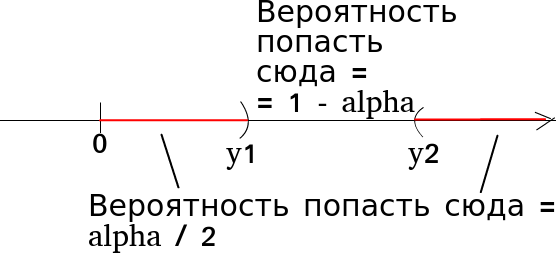
\includegraphics[width=.4\textwidth]{./pictures/10_3.png}
    \caption{Вероятность попадания в отрезок}
    \label{fig:103}
  \end{figure}

  Функция распределения будет иметь вид, показанный на рисунке \ref{fig:1031}.

  \begin{figure}[h!]
    \centering
    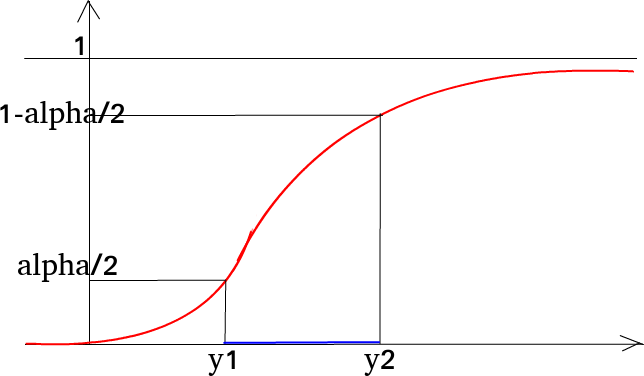
\includegraphics[width=.4\textwidth]{./pictures/10_3_1.png}
    \caption{Функция распределения}
    \label{fig:1031}
  \end{figure}

  $P \left( \xi \geq y_1 \wedge \xi \leq y_2 \right) = 1 - \alpha $.

  Подставляя вместо $ \xi $ выражение,
  можем определить интервал
  $$P \left( y_1 \leq \xi \leq y_2 \right) =
    1 - \alpha,$$
  то есть
  $$P \left\{ y_1 \leq \frac{ \left( n - 1 \right) \hat{ \sigma^2}}{ \sigma^2} \leq y_2 \right\} =
    1 - \alpha.$$

  Выражем пределы для нужной величины
  $$P \left\{
      \frac{1}{ \left( n - 1 \right) \hat{ \sigma^2}} \leq \frac{1}{ \sigma^2} \leq
      \frac{y_2}{ \left( n - 1 \right) \hat{ \sigma^2}}
    \right\} =
    1 - \alpha,$$
  получаем
  $$P \left\{
      \frac{ \left( n - 1 \right) \hat{ \sigma^2}}{y_2} = T_1 \leq
      \frac{ \left( n - 1 \right) \hat{ \sigma^2}}{y_1} = T_2
    \right\} =
    1 - \alpha.$$

  Получили выражение $P \left( T_1 \leq \sigma^2 \leq T_2 \right) = 1 - \alpha $, значит,
  $ \left[ T_1, T_2 \right] $ -- доверительный интеравал.
\end{enumerate}

\subsubsection*{10.4}

\textit{Задание.}
Пусть $X_1, \dotsc, X_n$ и $Y_1, \dotsc, Y_m$ --- две независимые выборки,
причём первая из них из распределения $N \left( a_1, \sigma_1^2 \right) $, а вторая ---
из распределения $N \left( a_2, \sigma_2^2 \right) $.
Постройте доверительный интервал для разности $a_1 - a_2$, считая,
что дисперсии являются известными.

\textit{Решение.} Известно, что
$$ \frac{ \sqrt{n} \left( \overline{X} - a_1 \right) }{ \sigma_1} \sim
  N \left( 0, 1 \right) $$
и
$$ \frac{ \sqrt{m} \left( \overline{Y} - a_2 \right) }{ \sigma_2} \sim
  N \left( 0, 1 \right).$$
Из этого следует, что
$$ \overline{X} - a_1 \sim
  N \left( 0, \frac{1}{n} \cdot \sigma_1^2 \right),$$
а
$$ \overline{Y} - a_2 \sim
  N \left( 0, \frac{1}{m} \cdot \sigma_2^2 \right).$$

Если рассмотрим разность, используем независимость выборок
$$ \left( \overline{X} - a_1 \right) - \left( \overline{Y} - a_2 \right) \sim
  N \left( 0, \frac{1}{n} \cdot \sigma_1^2 + \frac{1}{m} \cdot \sigma_2^2 \right).$$

Есть $ \xi \sim N \left( a_1, \sigma_1^2 \right) $ и $ \eta \sim N \left( a_2, \sigma_2^2 \right) $,
и они независимы.
Тогда
$$ \xi - \eta \sim
  N \left( a_1 - a_2, \sigma_1^2 + \sigma_2^2 \right).$$

Преобразуем разность выборок, чтобы получить стандартное нормальное распределение
$$ \frac{ \left( \overline{X} - a_1 \right) - \left( \overline{Y} - a_2 \right) }{ \sqrt{ \frac{ \sigma_1^2}{m} + \frac{ \sigma_2^2}{n}}} =
  \xi \sim
  N \left( 0, 1 \right),$$
а для его есть таблица значений.

Нужно теперь находить доверительный интервал (то же самое, что делали в пункте а) задачи 10.3).
$$P \left\{
    -u_{ \frac{ \alpha }{2}} \leq
    \frac{ \left( \overline{X} - a_1 \right) - \left( \overline{Y} - a_2 \right) }{ \sqrt{ \frac{ \sigma_1^2}{m} + \frac{ \sigma_2^2}{n}}} \leq
    u_{ \frac{ \alpha }{2}}
  \right\} =
  1 - \alpha.$$

Умножаем все части неравенства на знаменатель
$$P \left(
    -u_{ \frac{ \alpha }{2}} \sqrt{ \frac{ \sigma_1^2}{n} + \frac{\sigma_2^2}{m}} \leq
    u_{ \frac{ \alpha }{2}}
  \right) =
  1 - \alpha.$$

Выражем нужную разность
\begin{equation*}
  \begin{split}
    P \left(
      -u_{ \frac{ \alpha }{2}} \sqrt{ \frac{ \sigma_1^2}{n} + \frac{ \sigma_2^2}{m}} + \overline{X} -
      \overline{Y} = T_1 \leq
      a_1 - a_2 \leq
      u_{ \frac{ \alpha }{2}} \sqrt{ \frac{ \sigma_1^2}{n} + \frac{ \sigma_2^2}{m}} + \overline{X} -
      \overline{Y} = T_2
    \right) = \\
    = 1 - \alpha.
  \end{split}
\end{equation*}

Следовательно, $P \left( a_1 - a_2 \in \left[ T_1, T_2 \right] \right) = 1 - \alpha $.

\subsubsection*{10.5}

\textit{Задание.}
Пусть в условии предыдущей задачи все наблюдения имеют одинаковую, но неизвестную дисперсию,
то есть
$$X_i \sim N \left( a_1, \sigma^2 \right), \,
  Y_i \sim N \left( a_2, \sigma^2 \right).$$
Постройте доверительный интервал для разности $ \tau = a_1 - a_2$ средних.

\textit{Решение.}
\begin{equation*}
  \begin{split}
    \xi =
    \sqrt{ \frac{mn \left( m + n - 2 \right) }{m + n}} \cdot
    \frac{ \left( \overline{X} - a_1 \right) - \left( \overline{Y} - a_2 \right) }{ \sqrt{n \hat{ \sigma_1^2} + m \hat{ \sigma_2^2}}} =
    c \left[ \left( \overline{X} - a_1 \right) - \left( \overline{Y} - a_2 \right) \right] = \\
    = \frac{ \eta }{ \sqrt{ \frac{ \chi_{n + m - 2}^2}{n + m - 2}}} \sim
    t_{n + m - 2}.
  \end{split}
\end{equation*}

Видно, что в этой формуле $ \sigma^2$ нигде не участвует.
Здесь используется независимость выборок $X_1, \dotsc, X_n, Y_1, \dotsc, Y_m$.

Распределение Стьюдента симметрично,
поэтому можно искать одно число
$P \left( -u_{ \frac{ \alpha }{2}} \leq \xi \leq u_{ \frac{ \alpha }{2}} \right) =
  1 - \alpha $.

Подставляем значение случайной величины
$$P \left\{
    -u_{ \frac{ \alpha }{2}} \leq
    c \left[ \left( \overline{X} - a_1 \right) - \left( \overline{Y} - a_2 \right) \right] \leq
    u_{ \frac{ \alpha }{2}}
  \right\} =
  1 - \alpha.$$

Делим на константу
$$P \left(
    - \frac{u_{ \frac{ \alpha }{2}}}{c} \leq \overline{X} - a_1 - \overline{Y} + a_2 \leq
    \frac{u_{ \frac{ \alpha }{2}}}{c}
  \right) =
  1 - \alpha.$$

Переносим выборочные средние из центрального выражения неравенства
$$P \left(
    - \frac{u_{ \frac{ \alpha }{2}}}{c} - \overline{X} + \overline{Y} \leq - a_1 + a_2 \leq
    \frac{u_{ \frac{ \alpha }{2}}}{c} - \overline{X} + \overline{Y}
  \right) =
  1 - \alpha.$$

Умножаем на $-1$ все части неравенства и получаем доверительный интервал
$$P \left(
    - \frac{u_{ \frac{ \alpha }{2}}}{c} + \overline{X} - \overline{Y} = T_1 \leq - a_1 + a_2 \leq
    \frac{u_{ \frac{ \alpha }{2}}}{c} + \overline{X} - \overline{Y} = T_2
  \right) =
  1 - \alpha.$$

\subsubsection*{10.7}

\textit{Задание.}
Пусть $X_1, \dotsc, X_n$ ---
выборка из равномерного распределения на отрезке $ \left[ 0, \theta \right] $.
\begin{enumerate}[label=\alph*)]
  \item Докажите, что
  $$ \frac{X_{ \left( n \right) }}{ \theta }$$
  является центральной статистикой.
  \item Постройте доверительный интервал с уровнем доверия $1 - \alpha $ для параметра $ \theta $,
  используя центральную статистику.
\end{enumerate}

\textit{Решение.} $X_1, \dotsc, X_n \sim U \left( \left[ 0, \theta \right] \right) $.
\begin{enumerate}[label=\alph*)]
  \item Покажем, что
  $$ \frac{1}{ \theta } \cdot X_{ \left( n \right) } =
    G \left( \vec{X}, \theta \right).$$

  Функция монотонно убывает по $ \theta \in \Theta \in \left[ 0, + \infty \right) $.

  Ищем распределение
  $$F_{G \left( \vec{X}, \theta \right) } \left( y \right) =
    P \left\{ \frac{X_{ \left( n \right) }}{ \theta } \leq y \right\} =
    P \left\{ X_{ \left( n \right) } \leq y \theta \right\} =
    \left[ P \left( X_1 \leq y \theta \right) \right]^n.$$
  По определению функции распределения
  $$ \left[ P \left( X_1 \leq y \theta \right) \right]^n =
    F_{X_1} \left( y \theta \right)^n =
    \left(
      \int \limits_{- \infty }^y
        \frac{1}{ \theta } \cdot \mathbbm{1} \left\{ x \in \left[ 0, \theta \right] \right\}
      dx
    \right)^n.$$
  Выносим константу за знак интеграла и меняем пределы интегрирования за счёт индикатора
  $$ \left(
      \int \limits_{- \infty }^y
        \frac{1}{ \theta } \cdot \mathbbm{1} \left\{ x \in \left[ 0, \theta \right] \right\}
      dx
    \right)^n =
    \frac{1}{ \theta^n } \cdot
    \left( \int \limits_0^y \mathbbm{1} \left\{ x \leq \theta \right\} dx \right)^n.$$
  Рассматриваем 3 случая
  \begin{equation*}
    \begin{split}
      \frac{1}{ \theta^n } \cdot
      \left( \int \limits_0^y \mathbbm{1} \left\{ x \leq \theta \right\} dx \right)^n =
      \begin{cases}
        0, \qquad y < 0, \\
        \frac{1}{ \theta^n} \cdot
        \left( \int \limits_0^y \theta \cdot \mathbbm{1} \left\{ z \leq 1 \right\} dz \right)^n =
        \frac{1}{ \theta^n} \left( \int \limits_0^y \theta dz \right)^n = \\
        = y^n, \qquad y \in \left[ 0, 1 \right), \\
        1, \qquad y \geq 1.
      \end{cases}
    \end{split}
  \end{equation*}

  Можно найти распределение иначе
  $$ \frac{X_{ \left( n \right) }}{ \theta } =
    \frac{1}{ \theta } \cdot \max \left( X_1, \dotsc, X_n \right) =
    \max \left( \frac{X_1}{ \theta }, \dotsc, \frac{X_n}{ \theta } \right).$$
  Все случайные величины имеют одинаковое распределение
  $$ \max \left( \frac{X_1}{ \theta }, \dotsc, \frac{X_n}{ \theta } \right) \overset{d}{=}
    \max \left( \tilde{X_1}, \dotsc, \tilde{X_n} \right) =
    \tilde{X_{ \left( n \right) }} \sim
    U \left( \left[ 0, 1 \right] \right).$$
  \item Статистика
  $$ \frac{X_{ \left( n \right) }}{ \theta }$$
  имеет известное распределение.
  $$P \left\{ a_1 \leq \frac{X_{ \left( n \right) }}{ \theta } \leq a_2 \right\} \geq
    1 - \alpha.$$

  Делим на максимальную порядковую статистику
  $$P \left\{
      \frac{a_1}{X_{ \left( n \right) }} \leq \frac{1}{ \theta } \leq
      \frac{a_1}{X_{ \left( n \right) }}
    \right\} =
    P \left\{
      \frac{X_{ \left( n \right) }}{a_2} \leq \theta \leq \frac{X_{ \left( n \right) }}{a_1}
    \right\} \geq
    1 - \alpha,$$
  следовательно,
  $$ \left[ T_1, T_2 \right] =
    \left[ \frac{X_{ \left( n \right) }}{a_2}, \frac{X_{ \left( n \right) }}{a_1} \right].$$
\end{enumerate}

\addcontentsline{toc}{section}{Домашнее задание}
\section*{Домашнее задание}

\subsubsection*{10.9}

\textit{Задание.}
По реализации $2.96, 3.07, 3.02, 2.98, 3.06$
выборки объёма 5 из нормального распределения
с неизвестными параметрами постройте деверительные
интервалы для математического ожидания и дисперсии на уровне значимости $0.05$.

\textit{Решение.} Выборка имеет объём $n = 5$.

Найдём выборочное среднее
$$ \overline{X} =
  \frac{1}{5} \sum \limits_{i = 1}^5 X_i =
  \frac{2.96 + 3.07 + 3.02 + 2.98 + 3.06}{5} =
  3.018.$$

Найдём выборочную дисперсию
$$ \hat{ \sigma^2} =
  \frac{1}{4} \sum \limits_{i = 1}^5 \left( X_i - \overline{X} \right)^2.$$
Подставляем числа
\begin{equation*}
  \begin{split}
    \frac{1}{4} \sum \limits_{i = 1}^5 \left( X_i - \overline{X} \right)^2 = \\
    = \frac{1}{4} \left( 0.003364 + 0.002704 + 4 \cdot 10^{-6} + 0.001444 + 0.001764 \right) = \\
    = \frac{1}{4} \cdot 0.00928 =
    0.00232.
  \end{split}
\end{equation*}

Используем формулу
$$P \left(
    - \frac{ \sigma }{ \sqrt{n}} \cdot u_{ \frac{ \alpha }{2}} + \overline{X} \leq a \leq
    \frac{ \sigma }{ \sqrt{n}} \cdot u_{ \frac{ \alpha }{2}} + \overline{X}
  \right) =
  1 - \alpha =
  1 - 0.05 =
  0.95.$$

Из таблицы нормального распределения
$u_{ \frac{ \alpha }{2}} =
  u_{ \frac{0.05}{2}} =
  u_{0.025} =
  1.96$.

Ищем числовые выражения для пределов
$$- \frac{ \sigma }{ \sqrt{n}} \cdot u_{ \frac{ \alpha }{2}} + \overline{X} =
  - \frac{ \sqrt{0.00232}}{ \sqrt{5}} \cdot 1.96 + 3.018 =
  2.976$$
и
$$ \frac{ \sigma }{ \sqrt{n}} \cdot u_{ \frac{ \alpha }{2}} + \overline{X} =
  3.06.$$

Доверительный интервал для $a$ имеет вид $ \left[ 2.976, 3.06 \right] $.

Чтобы найти доверительный интервал для дисперсии, используем формулу
$$P \left\{
    \frac{ \left( n - 1 \right) \hat{ \sigma^2}}{X_2 \left( \alpha \right) } \leq \sigma^2 \leq
    \frac{ \left( n - 1 \right) \hat{ \sigma^2}}{X_1 \left( \alpha \right) }
  \right\} =
  1 - \alpha,$$
где $X_2 \left( \alpha \right)  = 11.7$ --- квантиль уровня
$$1 - \frac{ \alpha }{2}$$
с $n - 1$ степенью свободы, а $X_1 \left( \alpha \right) = 0.297$ --- квантиль уровня
$$ \frac{ \alpha }{2}$$
с $n - 1$ степенью свободы.

Тогда
$$ \frac{ \left( n - 1 \right) \hat{ \sigma^2}}{X_2 \left( \alpha \right) } =
  \frac{4 \cdot 0.00232}{11.7} =
  0.00079, \,
  \frac{ \left( n - 1 \right) \hat{ \sigma^2}}{X_1 \left( \alpha \right) } =
  \frac{4 \cdot 0.00232}{0.297} =
  0.03125.$$
Следовательно, доверительный интервал для $ \sigma^2$ имеет вид $ \left[ 0.00079, 0.03125 \right] $.

\subsubsection*{10.10}

\textit{Задание.}
Пусть $X_1, \dotsc, X_n$ и $Y_1, \dotsc, Y_n$ --- две независимые выборки,
причём первая из них из распределения $N \left( a_1, \sigma^2 \right) $, а вторая ---
из распределения $N \left( a_2, C \sigma^2 \right) $.
Постройте доверительный интервал для разности $ \tau = a_1 - a_2$,
считая параметры распределений неизвестными, а $C$ --- известным множителем.

\textit{Решение.}
$$ \xi =
  \sqrt{ \frac{nm \left( m + n - 2 \right) }{m + n}} \cdot
  \frac{ \left( \overline{X} - a_1 \right) - \left( \overline{Y} - a_2 \right) }{ \sqrt{n \hat{ \sigma_1^2} + mC \hat{ \sigma_2^2}}} =
  d \left[ \left( \overline{X} - a_1 - \overline{Y} - a_2 \right) \right].$$
Эта случайная величина имеет распределение $t_{m + n - 2}$.

Видим, что в этой формуле $ \sigma^2$ нигде не участвует.
Здесь используется независимость выборок $X_1, \dotsc, X_n, Y_1, \dotsc, Y_m$.

Распределение Стьюдента симметричное,
поэтому можно искать одно число
$P \left( -u_{ \frac{ \alpha }{2}} \leq \xi \leq u_{ \frac{ \alpha }{2}} \right) =
  1 - \alpha $.

Подставляем значение случайной величины
$$P \left\{
    -u_{ \frac{ \alpha }{2}} \leq
    d \left[ \left( \overline{X} - a_1 \right) - \left( \overline{Y} - a_2 \right) \right] \leq
    u_{ \frac{ \alpha }{2}}
  \right\} =
  1 - \alpha.$$

Делим на константу
$$P \left(
    - \frac{u_{ \frac{ \alpha }{2}}}{d} \leq \overline{X} - a_1 - \overline{Y} + a_2 \leq
    \frac{u_{ \frac{ \alpha }{2}}}{d}
  \right) =
  1 - \alpha.$$

Переносим выборочные средние из центрального выражения неравенства
$$P \left\{
    - \frac{u_{ \frac{ \alpha }{2}}}{d} - \overline{X} + \overline{Y} \leq
    - \left( a_1 - a_2 \right) \leq
    \frac{u_{ \frac{ \alpha }{2}}}{d} - \overline{X} + \overline{Y}
  \right\} =
  1 - \alpha.$$

Умножаем на -1 все части неравенства и получаем доверительный интервал
$$P \left(
    - \frac{u_{ \frac{ \alpha }{2}}}{d} + \overline{X} - \overline{Y} \leq
    - \left( a_1 - a_2 \right) \leq
    \frac{u_{ \frac{ \alpha }{2}}}{d} + \overline{X} - \overline{Y}
  \right) =
  1 - \alpha.$$
